\documentclass[
	10pt,								% globale Schriftgröße
	parskip=half-,						% setzt Absatzabstand hoch
	paper=a4,							% Format
	english,ngerman,					% lädt Sprachpakete
	]{scrartcl}							% Dokumentenklasse

% //////////////////// Pakete laden ////////////////////
\usepackage[fleqn]{amsmath}
\usepackage[fleqn]{mathtools}
\usepackage{amssymb}			% mathematische symbole, für \ceckmarks
\usepackage{amsthm}				% für proof
\usepackage{mathrsfs}			% für \mathscr
\usepackage{latexsym}
\usepackage{marvosym}				% für Lightning

\usepackage{fontspec} 			% funktioniert nur mit den neueren Compilern z.B. XeLaTeX
\usepackage{microtype}			% für bessere Worttrennung
\usepackage[ngerman]{babel} 	% Spracheinstellung
\usepackage{lmodern}			% verändert verwendete Schriftart, damit sie weniger pixelig ist

\usepackage{verbatim}
\usepackage{listings}			% Für Quellcode

\usepackage{graphicx}
\usepackage{tabularx}			% für Tabellen mit gleicher Spaltenbreite und automatischen Umbrüchen
\usepackage{fullpage}
\usepackage{multirow}			% für multirow in tabulars
\usepackage{rotate}
\usepackage[cmyk,table]{xcolor} % um Farben zu benutzen, kann mehr als das Paket color
\usepackage[					% Verlinkungen
	colorlinks,					% farbige Schrift, statt farbiger Rahmen
	linktocpage,				% verlinkt im Abb.Verzeichnis Seitenzahl statt Bildunterschrift
	linkcolor=blue				% setzt Farbe der Links auf blau
	]{hyperref}					% nur für digitale Anwendungen, url = "http://www.example.com"
\usepackage{url}				% für Webadressen wie e-mail usw.: "\url{http://www.example.com}"

\usepackage{enumerate}			% für versch. Aufzählungezeichen wie z.B. a)
\usepackage{xspace}				% folgt ein Leerzeichen nach einem \Befehl, wird es nicht verschluckt.
\usepackage{cancel}				% für das Durchstreichen u.a. in Matheformeln mit \cancel
\usepackage{float}              % zum Forcieren der Position von figure-Umgebungen

% zum Zeichnen (u.a. von Graphen)
\usepackage{fp}
\usepackage{tikz}
\usetikzlibrary{tikzmark}			% für \tikzmark{toRemember}
\usetikzlibrary{positioning}	% verbesserte Positionierung der Knoten
\usetikzlibrary{automata}		% für Automaten (GTI)
\usetikzlibrary{arrows}
\usetikzlibrary{shapes}
\usetikzlibrary{decorations.pathmorphing}
\usetikzlibrary{decorations.pathreplacing}
\usetikzlibrary{decorations.shapes}
\usetikzlibrary{decorations.text}

% //////////////////// Syntaxhighlighting ////////////////////
\lstloadlanguages{Python, Haskell, [LaTeX]TeX, Java}
\lstset{
   basicstyle=\footnotesize\ttfamily,	% \scriptsize the size of the fonts that are used for the code
   backgroundcolor = \color{bgcolour},	% legt Farbe der Box fest
   breakatwhitespace=false,	% sets if automatic breaks should only happen at whitespace
   breaklines=true,			% sets automatic line breaking
   captionpos=t,				% sets the caption-position to bottom, t for top
   commentstyle=\color{codeblue}\ttfamily,% comment style
   frame=single,				% adds a frame around the code
   keepspaces=true,			% keeps spaces in text, useful for keeping indentation
							% of code (possibly needs columns=flexible)
   keywordstyle=\bfseries\ttfamily\color{codepurple},% keyword style
   numbers=left,				% where to put the line-numbers;
   							% possible values are (none, left, right)
   numberstyle=\tiny\color{codegreen},	% the style that is used for the line-numbers
   numbersep=5pt,			% how far the line-numbers are from the code
   stepnumber=1,				% nummeriert nur jede i-te Zeile
   showspaces=false,			% show spaces everywhere adding particular underscores;
							% it overrides 'showstringspaces'
   showstringspaces=false,	% underline spaces within strings only
   showtabs=false,			% show tabs within strings adding particular underscores
   flexiblecolumns=false,
   tabsize=1,				% the step between two line-numbers. If 1: each line will be numbered
   stringstyle=\color{orange}\ttfamily,	% string literal style
   numberblanklines=false,				% leere Zeilen werden nicht mitnummeriert
   xleftmargin=1.2em,					% Abstand zum linken Layoutrand
   xrightmargin=0.4em,					% Abstand zum rechten Layoutrand
   aboveskip=2ex, 
}

\lstdefinestyle{py}{
   language=Python,
}
\lstdefinestyle{hs}{
   language=Haskell,
}
\lstdefinestyle{tex}{
	language=[LaTeX]TeX,
	escapeinside={\%*}{*)},     % if you want to add LaTeX within your code
	texcsstyle=*\bfseries\color{blue},% hervorhebung der tex-Schlüsselwörter
	morekeywords={*,$,\{,\},\[,\],lstinputlisting,includegraphics,
	rowcolor,columncolor,listoffigures,lstlistoflistings,
	subsection,subsubsection,textcolor,tableofcontents,colorbox,
	fcolorbox,definecolor,cellcolor,url,linktocpage,subtitle,
	subject,maketitle,usetikzlibrary,node,path,addbibresource,
	printbibliography},% if you want to add more keywords to the set
     numbers=none,
     numbersep=0pt,
     xleftmargin=0.4em,
}

\lstdefinestyle{java}{
	language=Java,
	extendedchars=true,		% lets you use non-ASCII characters;
   						% for 8-bits encodings only, does not work with UTF-8
}

\lstdefinelanguage[x64]{Assembler}     % add a "x64" dialect of Assembler
   [x86masm]{Assembler} % based on the "x86masm" dialect
   % with these extra keywords:
   {morekeywords={CDQE,CQO,CMPSQ,CMPXCHG16B,JRCXZ,LODSQ,MOVSXD, %
                  POPFQ,PUSHFQ,SCASQ,STOSQ,IRETQ,RDTSCP,SWAPGS, %
                  rax,rdx,rcx,rbx,rsi,rdi,rsp,rbp, %
                  r8,r8d,r8w,r8b,r9,r9d,r9w,r9b}
}					% for 8-bits encodings only, does not work with UTF-8

\lstdefinestyle{c}{
	language=c,
	extendedchars=true,		% for 8-bits encodings only, does not work with UTF-8
}

% //////////////////// eigene Kommandos ////////////////////
\newcommand\FU{Freie Universität Berlin\xspace}% benötigt package xspace
\newcommand\gdw{g.\,d.\,w.\xspace}
\newcommand\oBdA{o.\,B.\,d.\,A.\xspace}
\newcommand{\Eu}{\texteuro}
\newcommand\N{\mathbb{N}\xspace}
\newcommand\Q{\mathbb{Q}\xspace}
\newcommand\R{\mathbb{R}\xspace}
\newcommand\Z{\mathbb{Z}\xspace}
\newcommand\ohneNull{\ensuremath{\backslash\lbrace 0\rbrace}}% \{0}
\let\dhALT\dh	% Schreibt Befehl \dh in \dhALT um
\renewcommand\dh{d.\,h.\xspace}	%renew überschreibt command \dh
\newcommand\Bolt{\;\text{\LARGE\raisebox{-0.3em}{\Lightning}\normalsize}\xspace}% Blitz
\newcommand\zz{\ensuremath{\raisebox{+0.25ex}{Z}% zu zeigen
			\kern-0.4em\raisebox{-0.25ex}{Z}%
			\;\xspace}}
\newcommand{\from}{\ensuremath{\colon}}
\newcommand{\floor}[1]{\lfloor{#1}\rfloor}
\newcommand{\ceil}[1]{\lceil{#1}\rceil}
 \renewcommand{\L}{\ensuremath{\mathcal{L}}\xspace}
 \renewcommand{\P}{\ensuremath{\mathcal{P}}\xspace}
 \newcommand{\NL}{\ensuremath{\mathcal{N}\kern-0.2em\mathcal{L}}\xspace}
 \newcommand{\NP}{\ensuremath{\mathcal{NP}}\xspace}

% //////////////////// Mathefunktionen ////////////////////
\DeclareMathOperator{\Landau}{\mathcal{O}}
\DeclareMathOperator{\True}{True}
\DeclareMathOperator{\False}{False}

% //////////////////// eigene Theoreme ////////////////////
\newtheorem{theorem}{Satz}
\newtheorem{corollary}[theorem]{Folgerung}
\newtheorem{lemma}[theorem]{Lemma}
\newtheorem{observation}[theorem]{Beobachtung}
\newtheorem{definition}[theorem]{Definition}
\newtheorem{Literatur}[theorem]{Literatur}
% konfiguriert proof
\makeatletter
\newenvironment{Proof}[1][\proofname]{\par
  \pushQED{\qed}%
  \normalfont \topsep6\p@\@plus6\p@\relax
  \trivlist
  \item[\hskip\labelsep
%         \itshape
        \bfseries
    #1\@addpunct{.}]\ignorespaces
}{%
  \popQED\endtrivlist\@endpefalse
}
\makeatother

% //////////////////// eigene Farben ////////////////////
\let\definecolor=\xdefinecolor
\definecolor{FUgreen}{RGB}{153,204,0}
\definecolor{FUblue}{RGB}{0,51,102}

\definecolor{middlegray}{rgb}{0.5,0.5,0.5}
\definecolor{lightgray}{rgb}{0.8,0.8,0.8}
\definecolor{orange}{rgb}{0.8,0.3,0.3}
\definecolor{azur}{rgb}{0,0.7,1}
\definecolor{yac}{rgb}{0.6,0.6,0.1}
\definecolor{Pink}{rgb}{1,0,0.6}

\definecolor{bgcolour}{rgb}{0.97,0.97,0.97}
\definecolor{codegreen}{rgb}{0,0.6,0}
\definecolor{codegray}{rgb}{0.35,0.35,0.35}
\definecolor{codepurple}{rgb}{0.58,0,0.82}
\definecolor{codeblue}{rgb}{0.4,0.5,1}

% //////////////////// eigene Settings ////////////////////

\textheight = 230mm		% Höhe des Satzspiegels / Layouts
\footskip = 10ex			% Abstand zw. Fußzeile und Grundlinie letzter Textzeile
\parindent 0pt			% verhindert Einrückung der 1. Zeile eines Absatzes
\setkomafont{sectioning}{\rmfamily\bfseries}% setzt Ü-Schriften in Serifen, {disposition}											% bindet Header ein (WICHTIG)
\usepackage{graphicx}
\usepackage{amsmath}
\usepackage{amssymb}
\usepackage{fancyvrb}

\newcommand{\dozent}{Prof. R. Rojas}					% <-- Names des Dozenten eintragen
\newcommand{\projectNo}{5}
\newcommand{\veranstaltung}{Mustererkennung}
\newcommand{\semester}{WS17/18}
\newcommand{\studenten}{Boyan Hristov, Nedeltscho Petrov}
% /////////////////////// BEGIN DOKUMENT /////////////////////////


\begin{document}
% /////////////////////// BEGIN TITLEPAGE /////////////////////////
\begin{titlepage}
	\subject{\dozent}
	\title{\veranstaltung, \semester}
	\subtitle{\Large Übungsblatt \projectNo\\ \large\vspace{1ex} }
	\author{\studenten}
	\date{\normalsize \today}
\end{titlepage}

\maketitle								% Erstellt das Titelblatt
\vspace*{-9cm}							% rückt Logo an den oberen Seitenrand
\makebox[\dimexpr\textwidth+1cm][r]{	%rechtsbündig und geht rechts 1cm über Layout hinaus
	
\includegraphics[width=0.4\textwidth]{src/fu_logo} % fügt FU-Logo ein
}
% /////////////////////// END TITLEPAGE /////////////////////////

\vspace{7cm}							% Abstand
\rule{\linewidth}{0.8pt}				% horizontale Linie										% erstellt die Titelseite


Link zum Git Repository: \url{https://github.com/BoyanH/FU-MachineLearning-17-18/tree/master/Solutions/Homework\projectNo}

\section*{Expectation Maximization}

Das Verfahren is für gestreute Datensätze eine deutlich bessere Clustering Methode als K-Means. Viel, womit wir das
vergleichen können, haben wir noch nicht gelern. Für den gegebenen Datensatz, der zwei sehr stark ausgeprägte Clusters
hat, hat es aber super funktioniert. Wir erkennen aber die Clusters nur anhand der Streuung der Daten, d.h also wir
wurden Schwierigkeiten mit K-Means haben, selbe Ergebsnisse zu bekommen.

\section*{Plots}

Wir haben das durchscnittliche Distanz zum Cluster (Mahalanobis) von allen Punkten abhängig von den Anzahl der Cluster.
Damit die Graphik besser aussieht, haben wir scipy benutz, es existiert aber natürlich kein Clustering mit z.B. 2.3
Cluster.

Auf dem Plot kann man die im Tutorium besprochene "Elbow" leider nicht sehen. Es war nur in einer früheren Version
des Programms zu sehen, die ähnlicher zu K-Means war. Es liegt vermutlich daran, dass den Datensatz eine größe und
leicht erkennbare Streuung der Daten hat. Nachdem man mehr als 2 Cluster versucht zu finden, werden viele Punkte
außerhalb des Streuungsbereichs eines Clusters liegen, aber trotzdem zu dem Cluster gehören. Das ist so, da je mehr
man die Daten splitted in mehreren Clusters, desto weniger wichtig wird die Streuung eines Clusters verglichen mit einem
anderen. Naja, "long story short" wird denken 2 Clusters sind am bestens geeignet für diesen Datensatz.

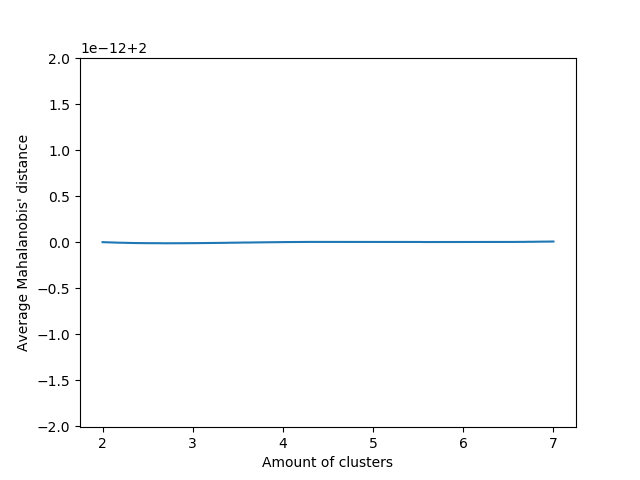
\includegraphics[width=\textwidth]{./plots/avrg_distance_for_k.png}

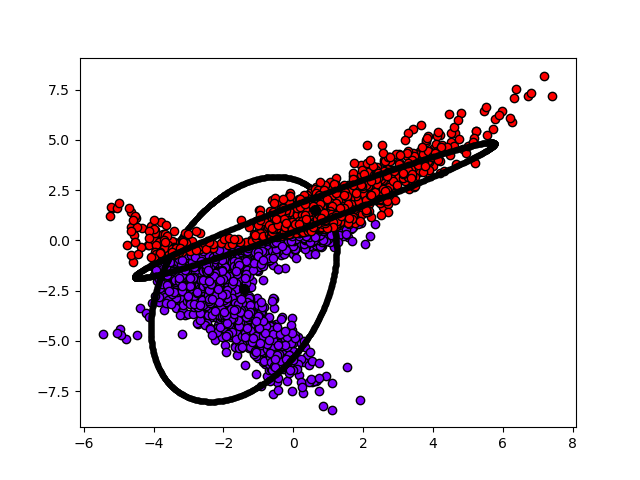
\includegraphics[width=\textwidth]{./plots/plot_for_k_2.png}

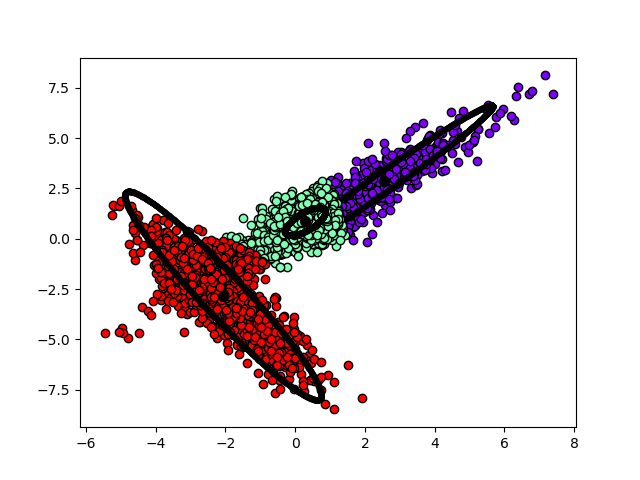
\includegraphics[width=\textwidth]{./plots/plot_for_k_3.png}

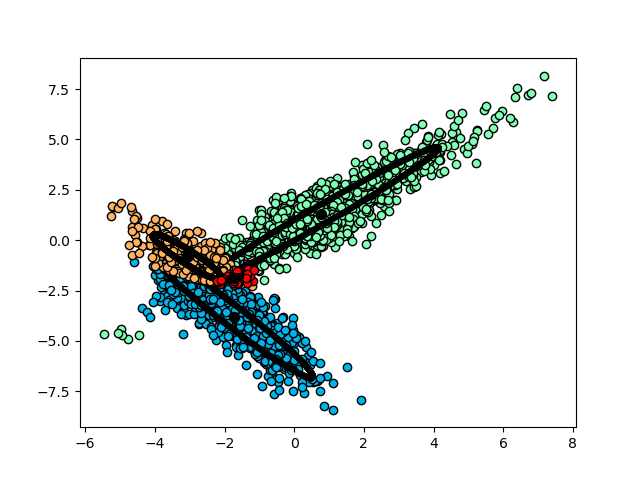
\includegraphics[width=\textwidth]{./plots/plot_for_k_5.png}

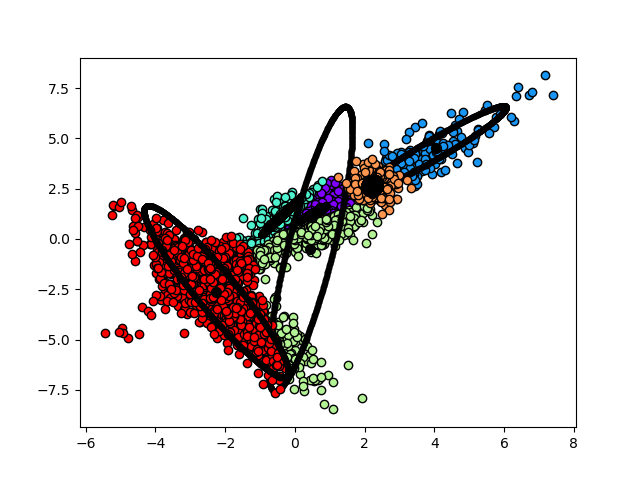
\includegraphics[width=\textwidth]{./plots/plot_for_k_6.png}

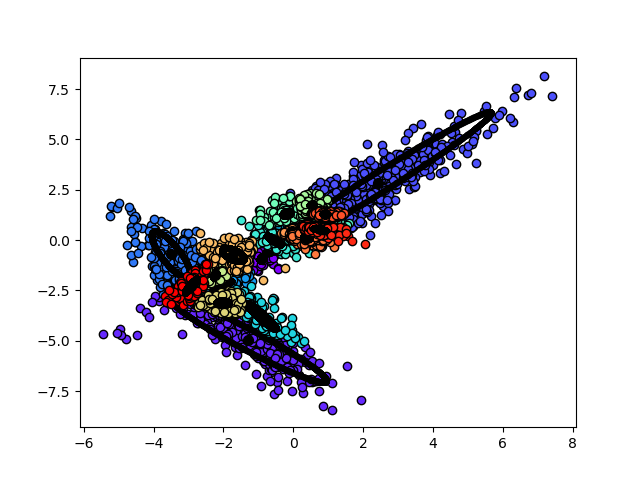
\includegraphics[width=\textwidth]{./plots/plot_for_k_20.png}


\section*{Details zur Implementierung}

Interessant für die Implementierung sind wahrscheinlich die Berechnung von dem Abstand und die Entscheidung,
wann der Algorithmus eigentlich fertig ist.


Mahalanobis Abstand - wir könnten uns hier den Wurzel sparen, so haben wir aber deutlich präziseren
durchschnittlichen Abstand bekommen, der besser zu plotten war. Da sonst die Großteil der Implementierung
vektorisiert ist, hatten wir nicht zu viele Sorgen wegen Performance. Sehr interessant ist es eigentlich nicht,
nur die Formel aus der Vorlesung..

\begin{lstlisting}[style=py]
    def get_distance_mahalanobis_to_cluster(self, x, i_cluster):
        # the square root could be removed, but helps for better plotting
        return math.sqrt((x - self.cluster_centers[i_cluster]).dot(
            self.inv_covariances_per_cluster[i_cluster]).dot((x - self.cluster_centers[i_cluster]).T))
\end{lstlisting}



Cluster Zentren berechnen, vektorisiert
\begin{lstlisting}[style=py]
    def calculate_cluster_centers(self):
        get_cluster_centers = np.vectorize(lambda x, points_per_center: points_per_center[x].mean(0),
                                           signature='(),(m)->(n)')
        self.cluster_centers = get_cluster_centers(self.cluster_indexes, self.points_per_cluster)
\end{lstlisting}


Berechnung von Kovarianzmatrizen - dafür haben wir Numpy benutzt, interessant es aber der Fall, wenn wir nicht genug
Punkte haben. Dann nehmen wir bloß die Identitätsmatrix. "again" steht im Kommentare, da wir bei der Initialisierung
auch die Identitätsmatrix nehmen.
\begin{lstlisting}[style=py]
    def calculate_covariances(self):
        # if we only have the center in our cluster (empty cluster) then just use the identity
        # matrix as covariance matrix again
        get_covariances = np.vectorize(lambda x, points_for_cluster: np.cov(points_for_cluster[x],
                                        rowvar=False, bias=True) if len(points_for_cluster[x]) > 1 else
                                        np.identity(len(points_for_cluster[x][0])), signature='(),(m)->(n,n)')
        self.covariances_per_cluster = get_covariances(self.cluster_indexes, self.points_per_cluster)
        self.inv_covariances_per_cluster = np.vectorize(lambda x: np.linalg.pinv(x),
                                                        signature='(m,n)->(m,n)')(self.covariances_per_cluster)
\end{lstlisting}


"Main" Methode - wir haben hier anhand von Flags zwie Vorgehensweisen implementiert. Entweder terminiert man,
wenn die Clusterzentren sich nicht so viel bewegen, oder falls man 1. schlechtere Ergebnisse bekommt oder 2.
ein Wunschergebniss erreicht hat. In beiden Implementierungen gibt es eine maximale Anzahl von Iterationen (30, vermutlich
wäre 10 besser, aber... ^^)
\begin{lstlisting}[style=py]
    def apply_expectation_maximization(self, k=0):
        if VERBOSE:
            print('iteration: {}'.format(k))
        old_centers = np.copy(self.cluster_centers)
        old_distance = np.copy(self.mean_distance)
        self.reset_points_per_cluster()
        self.assign_points_to_clusters()
        self.calculate_cluster_centers()
        self.calculate_covariances()
        self.update_mean_distance_to_cluster_centers()

        # for some reason old_distance is None or old_distance > ...
        # was throwing errors cannot compare NoneType with int
        # therefore the less readable not old_distance :X

        # but basically, if judging on distance for when to stop,
        # if the average distance gets worse, we reach the max amount of iterations or we reach our desired
        # threshold, stop
        if USE_DISTANCE_THRESHOLD:
            if (self.mean_distance > DISTANCE_THRESHOLD and
                        k < self.max_iterations and (not old_distance or old_distance > self.mean_distance)):
                self.apply_expectation_maximization(k + 1)

        # other method to determine when to stop is by simply checking if the cluster centers still move enough
        elif abs((old_centers - self.cluster_centers).sum()) > MOVEMENT_THRESHOLD and k < self.max_iterations:
            self.apply_expectation_maximization(k + 1)
\end{lstlisting}


\section*{Vollständiges Code zu Expectation Maximization}
\begin{lstlisting}[style=py]
from Parser import parse_data
import numpy as np
from Helpers import save_plot, plot_covariance
from random import random
import matplotlib.pyplot as plt
import matplotlib.cm as cm
from scipy.interpolate import spline
import random
import math

CHOOSE_INITIAL_CENTERS_RANDOMLY = True
USE_DISTANCE_THRESHOLD = True
MOVEMENT_THRESHOLD = 0.002
DISTANCE_THRESHOLD = 0.01

VERBOSE = False
PLOT_MEAN_FOR_CLUSTERS_COUNT = True
PLOT_CLUSTERING_FOR_SOME_K = True
SAVE_PLOTS = True


class ExpectationMaximization:
    @staticmethod
    def get_initial_centers_from_data_set(data, k):
        if CHOOSE_INITIAL_CENTERS_RANDOMLY:
            random.seed(8)
            return np.array(random.choices(data, k=k), dtype=np.float64)

        min_point = data.min(0)
        max_point = data.max(0)
        centers = []

        for i in range(k):
            centers.append(min_point + (max_point - min_point) / k)

        return centers

    def __init__(self):
        self.data = None
        self.k_clusters = None
        self.sigma = None
        self.cluster_centers = None
        self.points_per_cluster = None
        self.inv_covariances_per_cluster = []
        self.covariances_per_cluster = []
        self.cluster_indexes = None
        self.last_diff = None
        self.mean_distance = None
        self.max_iterations = None

    def reset_points_per_cluster(self):
        self.points_per_cluster = [[x] for x in self.cluster_centers]

    def cluster(self, data, k_clusters, max_iterations=30):
        self.data = data
        self.mean_distance = None
        self.last_diff = None
        self.k_clusters = k_clusters
        self.cluster_indexes = [x for x in range(self.k_clusters)]
        self.cluster_centers = ExpectationMaximization.get_initial_centers_from_data_set(data, k_clusters)
        self.covariances_per_cluster = [[np.identity(len(x))] for x in self.cluster_centers]
        self.inv_covariances_per_cluster = self.covariances_per_cluster
        self.reset_points_per_cluster()
        self.max_iterations = max_iterations
        self.apply_expectation_maximization()

    def apply_expectation_maximization(self, k=0):
        if VERBOSE:
            print('iteration: {}'.format(k))
        old_centers = np.copy(self.cluster_centers)
        old_distance = np.copy(self.mean_distance)
        self.reset_points_per_cluster()
        self.assign_points_to_clusters()
        self.calculate_cluster_centers()
        self.calculate_covariances()
        self.update_mean_distance_to_cluster_centers()

        # for some reason old_distance is None or old_distance > ...
        # was throwing errors cannot compare NoneType with int
        # therefore the less readable not old_distance :X

        # but basically, if judging on distance for when to stop,
        # if the average distance gets worse, we reach the max amount of iterations or we reach our desired
        # threshold, stop
        if USE_DISTANCE_THRESHOLD:
            if (self.mean_distance > DISTANCE_THRESHOLD and
                        k < self.max_iterations and (not old_distance or old_distance > self.mean_distance)):
                self.apply_expectation_maximization(k + 1)

        # other method to determine when to stop is by simply checking if the cluster centers still move enough
        elif abs((old_centers - self.cluster_centers).sum()) > MOVEMENT_THRESHOLD and k < self.max_iterations:
            self.apply_expectation_maximization(k + 1)

    def update_mean_distance_to_cluster_centers(self):
        # 1. get distance for every point in each cluster in a single array
        # 2. get mean of that

        dis_for_x_in_k = np.vectorize(lambda x, i: self.get_distance_mahalanobis_to_cluster(x, i),
                                      signature='(m),()->()')

        # didn't manage to vectorize this one ;/ somehow, numpy doens't like jagged arrays
        distances_for_points = list(map(lambda x: dis_for_x_in_k(self.points_per_cluster[x], x),
                                        self.cluster_indexes))

        flattened_distances = []
        for cluster_distances in distances_for_points:
            flattened_distances = flattened_distances + list(cluster_distances)

        self.mean_distance = np.array(flattened_distances, dtype=np.float64).mean()

        if VERBOSE:
            print('Average Mahalanobis\' distance to cluster center: {}'.format(self.mean_distance))

    def assign_points_to_clusters(self):
        assign_points_to_clusters = np.vectorize(lambda x: self.assign_point_to_cluster(x),
                                                 signature='(m)->()')
        assign_points_to_clusters(self.data)

        for idx, list in enumerate(self.points_per_cluster):
            self.points_per_cluster[idx] = np.array(self.points_per_cluster[idx])

    def assign_point_to_cluster(self, point):
        distances_to_clusters = [self.get_distance_mahalanobis_to_cluster(point, i) for i in self.cluster_indexes]
        closest_cluster_idx = np.argmin(distances_to_clusters)
        self.points_per_cluster[closest_cluster_idx].append(point)

    def get_distance_mahalanobis_to_cluster(self, x, i_cluster):
        # the square root could be removed, but helps for better plotting
        return math.sqrt((x - self.cluster_centers[i_cluster]).dot(
            self.inv_covariances_per_cluster[i_cluster]).dot((x - self.cluster_centers[i_cluster]).T))

    def calculate_cluster_centers(self):
        get_cluster_centers = np.vectorize(lambda x, points_per_center: points_per_center[x].mean(0),
                                           signature='(),(m)->(n)')
        self.cluster_centers = get_cluster_centers(self.cluster_indexes, self.points_per_cluster)

    def calculate_covariances(self):
        # if we only have the center in our cluster (empty cluster) then just use the identity
        # matrix as covariance matrix again
        get_covariances = np.vectorize(lambda x, points_for_cluster: np.cov(points_for_cluster[x],
                                        rowvar=False, bias=True) if len(points_for_cluster[x]) > 1 else
                                        np.identity(len(points_for_cluster[x][0])), signature='(),(m)->(n,n)')
        self.covariances_per_cluster = get_covariances(self.cluster_indexes, self.points_per_cluster)
        self.inv_covariances_per_cluster = np.vectorize(lambda x: np.linalg.pinv(x),
                                                        signature='(m,n)->(m,n)')(self.covariances_per_cluster)


data = parse_data()
em = ExpectationMaximization()

# Depending on the cluster centers that are chosen, results differ
# Though mostly between 3 and 4 clusters fit best for the current data set
if PLOT_MEAN_FOR_CLUSTERS_COUNT:
    cluster_count_experiments = [x for x in range(2, 20)]
    cluster_count_mean_distance_results = []

    for cluster_count in cluster_count_experiments:
        em.cluster(data, cluster_count)
        cluster_count_mean_distance_results.append(np.copy(em.mean_distance))

        if VERBOSE:
            for idx, points in enumerate(em.points_per_cluster):
                print('Points in cluster #{}: {}'.format(idx, len(points)))

    x = np.linspace(min(cluster_count_experiments), max(cluster_count_experiments), 300)
    y = spline(cluster_count_experiments, cluster_count_mean_distance_results, x)

    figure = plt.figure()
    plt.plot(x, y)
    plt.xlabel('Amount of clusters')
    plt.ylabel('Average Mahalanobis\' distance')

    if SAVE_PLOTS:
        save_plot(figure, './plots/avrg_distance_for_k.png')
    else:
        plt.show()

if PLOT_CLUSTERING_FOR_SOME_K:
    plot_for_k_s = [2,3,5,6, 20]
    # plot_for_k_s = [2]

    for k in plot_for_k_s:
        em.cluster(data, k)
        colors = cm.rainbow(np.linspace(0, 1, k))

        fig = plt.figure()
        ax1 = fig.add_subplot(111)

        for cl_idx in em.cluster_indexes:
            X = em.points_per_cluster[cl_idx]
            x, y = zip(*X)
            # ax1.figure(figsize=(15, 10))
            ax1.scatter(x, y, edgecolors="black", c=colors[cl_idx])

            center = em.cluster_centers[cl_idx]
            covariance = em.covariances_per_cluster[cl_idx]
            plot_covariance(ax1, center[0], center[1], covariance)

        if SAVE_PLOTS:
            save_plot(fig, './plots/plot_for_k_{}.png'.format(k))
        else:
            plt.show()




# Parser.py

import csv
import numpy as np
import os
from sklearn.model_selection import train_test_split


def parse_data():
    file_name = os.path.join(os.path.dirname(__file__), './Dataset/2d-em.csv')
    csv_file = open(file_name, 'rt')
    reader = csv.reader(csv_file, delimiter=',', quoting=csv.QUOTE_NONE)

    return np.array([row for row in reader], dtype=np.float64)





# Helpers.py

import os
import pandas as pd
from numpy import pi, sin, cos
import numpy as np
import matplotlib.pyplot as plt

RGB_BLACK = [0, 0, 0]


def save_plot(fig, path):
    fig.savefig(os.path.join(os.path.dirname(__file__), path))


def plot_covariance(ax1, x_initial, y_initial, cov):
    num_points = 1000
    radius = 1.5  # adjusted radius, seems more correct this way

    # plot a circle
    arcs = np.linspace(0, 2 * pi, num_points)
    x = radius * sin(arcs)
    y = radius * cos(arcs)

    # stretch it according to the covariance matrix
    xy = np.array(list(zip(x, y)))
    x, y = zip(*xy.dot(cov))

    # move it in the space so it's center is above the cluster's center
    x = x + x_initial
    y = y + y_initial

    ax1.scatter(x, y, c=RGB_BLACK, s=10)  # plot covariance
    ax1.scatter([x_initial], [y_initial], c=RGB_BLACK, s=50)  # plot center

\end{lstlisting}



\begin{lstlisting}[style=py]

\end{lstlisting}



\begin{lstlisting}[style=py]

\end{lstlisting}



\begin{lstlisting}[style=py]

\end{lstlisting}



\begin{lstlisting}[style=py]

\end{lstlisting}



\begin{lstlisting}[style=py]

\end{lstlisting}


% /////////////////////// END DOKUMENT /////////////////////////
\end{document}
